\section{Conservation Tracking}

\begin{frame}{Concept}
    \begin{figure}
        \centering
        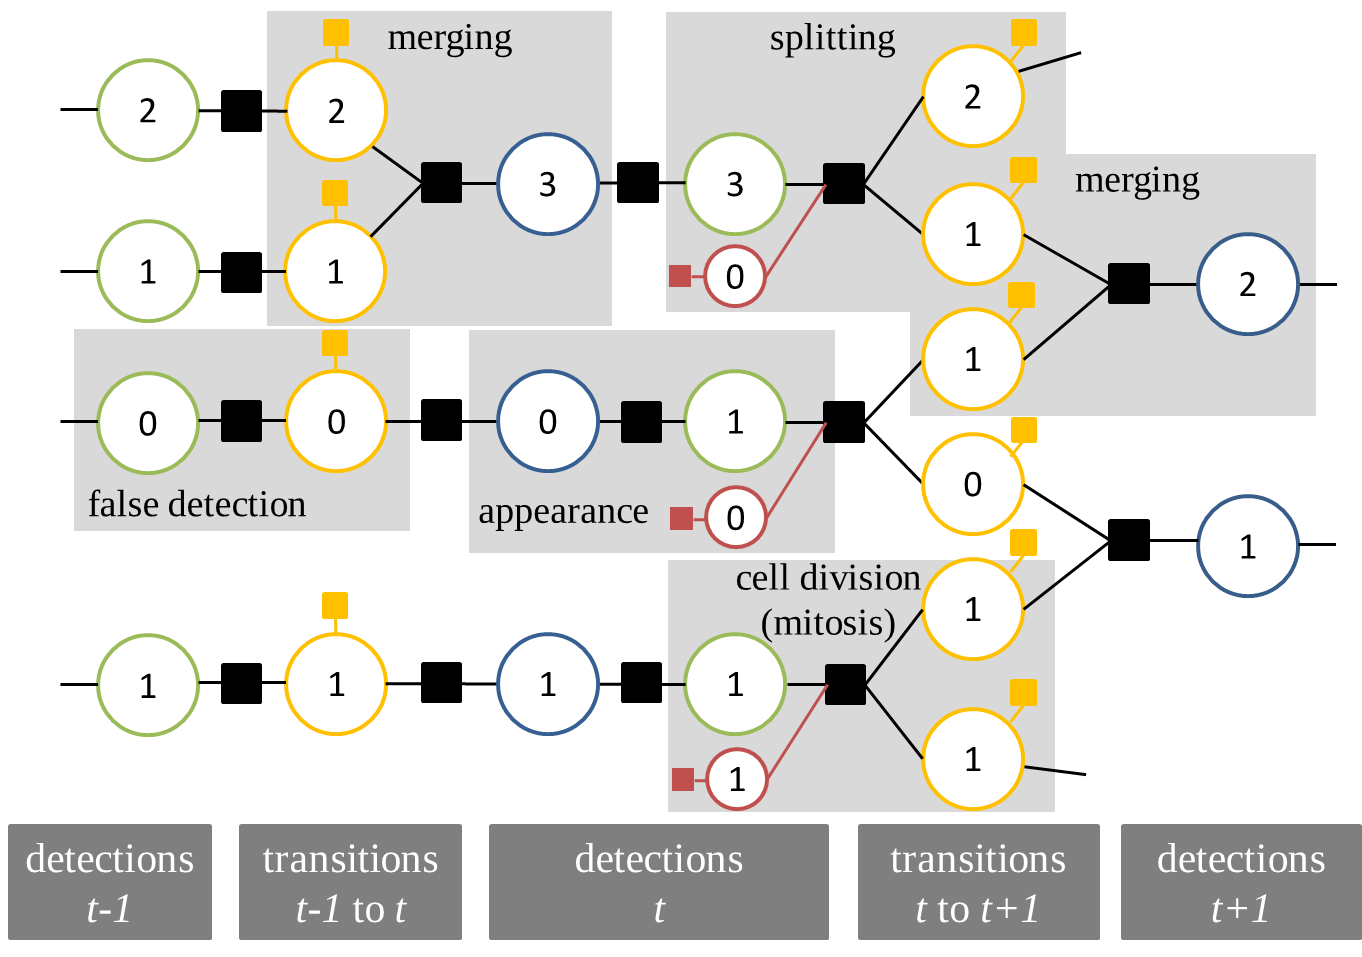
\includegraphics[width=0.8\textwidth]{images/conservation/factor_graph_big3.png}
        \caption{[Schiegg \etal (2013): Conservation Tracking]}
    \end{figure}
\end{frame}

\begin{frame}{Concept}
    \begin{tikzpicture}
        \node[label=left:$t\phantom{+1}$] (s1)
        {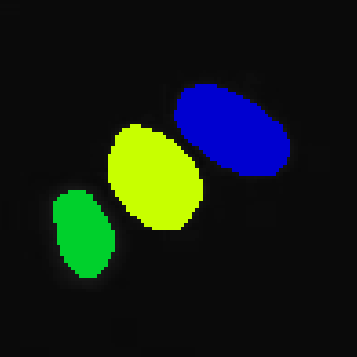
\includegraphics[width=0.17\textwidth]{images/conservation/concept/chaingraph-01.png}};
        \node[label=left:$t+1$, below=of s1.center] (s2)
        {
\includegraphics[width=0.17\textwidth]{images/conservation/concept/chaingraph-02.png}};
        \node[label=left:$t+2$, below=of s2.center] (s3)
        {
\includegraphics[width=0.17\textwidth]{images/conservation/concept/chaingraph-03.png}};
        \node[above=of s1.center] {Segmentation};
        \uncover<2->{
            \node[right=of s1.center, xshift=12pt] (t1)
            {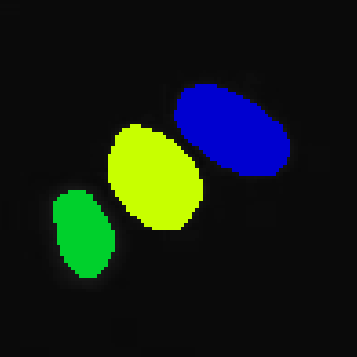
\includegraphics[width=0.17\textwidth]{images/conservation/concept/constracking-01.png}};
            \node[ below=of t1.center] (t2)
            {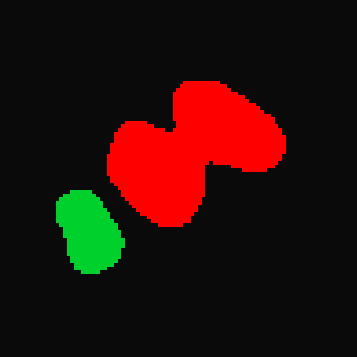
\includegraphics[width=0.17\textwidth]{images/conservation/concept/constracking-02.png}};
            \node[below=of t2.center] (t3)
            {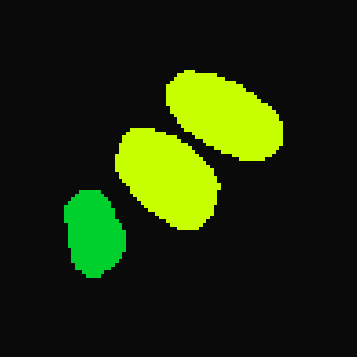
\includegraphics[width=0.17\textwidth]{images/conservation/concept/constracking-03.png}};
            \node[above=of t1.center] {Tracking};
            \node[font=\boldmath, yshift=2pt] at (t2.center) {$2$};
        }
        \uncover<3->{
            \node[right=of t1.center, xshift=12pt] (m1)
            {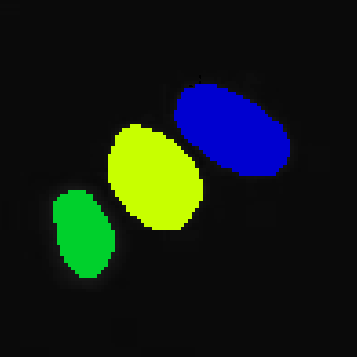
\includegraphics[width=0.17\textwidth]{images/conservation/concept/resolution-01.png}};
            \node[ below=of m1.center] (m2)
            {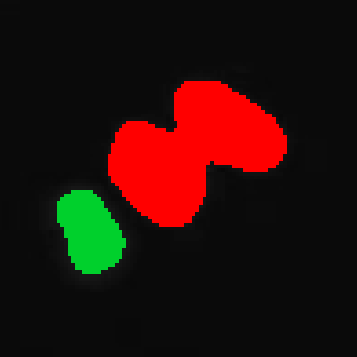
\includegraphics[width=0.17\textwidth]{images/conservation/concept/resolution-02.png}};
            \node[below=of m2.center] (m3)
            {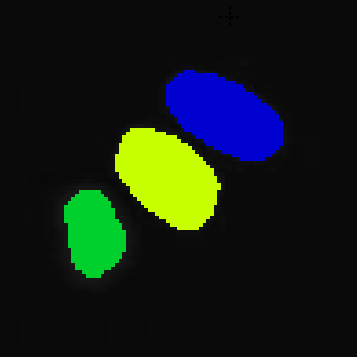
\includegraphics[width=0.17\textwidth]{images/conservation/concept/resolution-03.png}};
            \node[above=of m1.center, align=center] {Resolved\\Mergers};
            \node[font=\boldmath, yshift=2pt] at (m2.center) {$2$};
        }
    \end{tikzpicture}
\end{frame}

\begin{frame}{Workflow}
    \begin{figure}
        \centering
        \begin{tikzpicture}
            \node[anchor=south west, inner sep=0] (image) at (0,0)
            {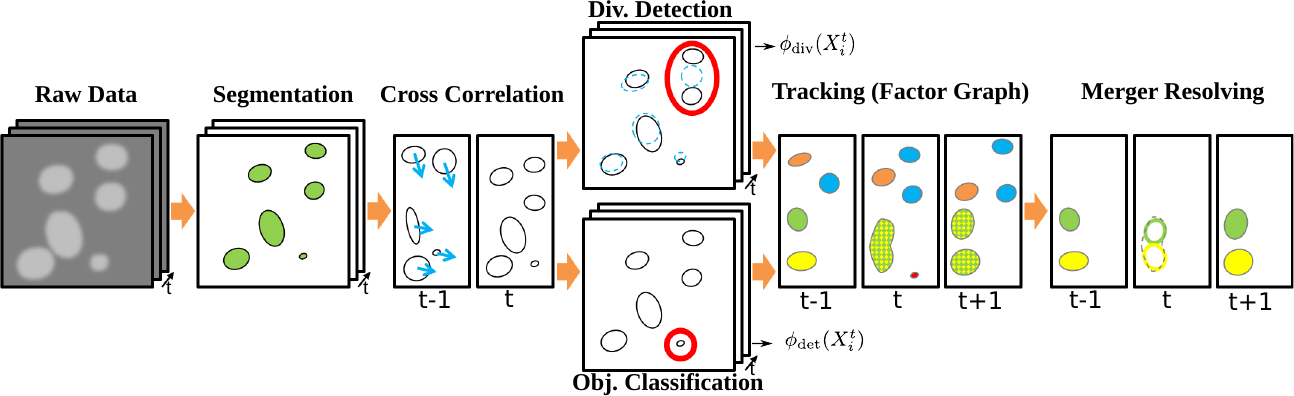
\includegraphics[width=\textwidth]{images/conservation/pipeline.png}};
            \begin{scope}[x={(image.south east)},y={(image.north west)}]
                \draw[red,line width=2pt,rounded corners, fill=red!20, fill opacity=0.3]
                (0.81,0.20) rectangle (1.003,0.83);
            \end{scope}
        \end{tikzpicture}

        \label{fig:conservation-pipeline}
    \end{figure}
\end{frame}

% \begin{frame}{Factor Graph}
%     \begin{figure}
%         \centering
%         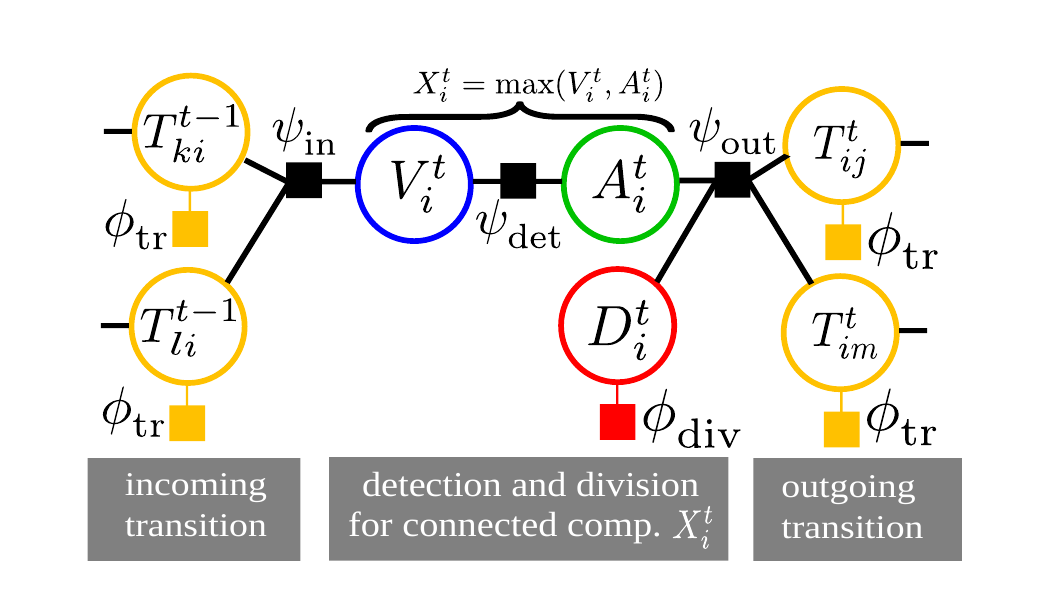
\includegraphics[width=\textwidth]{images/conservation/factor_graph.png}
%         \caption{Graphical model of the conservation tracking. [SOURCE]}
%         \label{fig:conservation-fg}
%     \end{figure}
% \end{frame}

\begin{frame}{Merger Resolution - Gaussian Mixture Model}
    \begin{figure}
        \centering
        \begin{subfigure}[b]{0.44\textwidth}
            \centering
            \scalebox{0.74}{
                % \begin{tikzpicture}
% \tikzstyle{main}=[circle, minimum size = 10mm, thick, draw =black!80, node distance = 16mm]
% \tikzstyle{hyparam}=[rectangle, minimum size = 5mm, thick, draw =black!80, fill = black!10, node distance = 16mm]
% \tikzstyle{param}=[rectangle, minimum size = 5mm, thick, draw =black!80, node distance = 16mm]
% \tikzstyle{connect}=[-latex, thick]
% \tikzstyle{selector}=[-latex, -|, snake=snake,segment amplitude=.4mm,segment length=2mm,line after snake=1mm, thick]
% \tikzstyle{shortconnect}=[-latex, thin]
% \tikzstyle{box}=[rectangle, draw=black!100]
% \tikzstyle{switch}=[circle, minimum size = 1mm, fill = black!100, draw=black!100]
%   \node[param] (phi) [label=below:$p(h)$] {$[H]$};
%   \node[main] (z) [right of=phi,label=below:$h^n$] {K};
%   \node[param] (mu) [above of=phi,yshift=10mm, label=below:$\MUH$] { };
%   \node[main, fill = black!10] (x) [right of= z,label=below:$v^n$] { };
%   \node[param] (sigma) [above of=z,yshift=10mm, label=right:$\SIGMAH$] { };
%   \path (phi) edge [connect] (z)
%         (z) edge [selector] (x)
%         (mu) edge [connect] (x)
%         (sigma) edge [connect] (x);
%   \node[rectangle, inner sep=0mm, fit= (z) (x),label=below right:$N$, xshift=9mm] {};
%   \node[rectangle, inner sep=4.4mm,draw=black!100, fit= (z) (x), xshift=1mm] {};
%   \node[rectangle, inner sep=2mm, fit= (mu) (sigma),label=below right:$H$, yshift=-2mm, xshift=11mm] {};
%   \node[rectangle, inner sep=6.4mm,draw=black!100, fit= (mu) (sigma), yshift=-2mm, xshift=3mm] {};
% \end{tikzpicture}

\begin{tikzpicture}
  \node[param] (pi) [] {$\Pi$};
  \node[main] (z) [right of=pi,label=below:$h^n$] { };
  \node[param] (mu) [above of=pi,yshift=10mm, label=below:$\MUH$] { };
  \node[main, fill = black!30] (x) [right of= z,label=below:$v^n$] { };
  \node[param] (sigma) [above of=z,yshift=10mm, label=right:$\SIGMAH$] { };
  \path (pi) edge [connect] (z)
        (z) edge [connect] (x)
        (mu) edge [connect] (x)
        (sigma) edge [connect] (x);
  \node[rectangle, inner sep=0mm, fit= (z) (x),label=below right:N, xshift=9mm] {};
  \node[rectangle, inner sep=4.4mm,draw=black!100, fit= (z) (x), xshift=1mm] {};
  \node[rectangle, inner sep=2mm, fit= (mu) (sigma),label=below right:H, yshift=-2mm, xshift=11mm] {};
  \node[rectangle, inner sep=6.4mm,draw=black!100, fit= (mu) (sigma), yshift=-2mm, xshift=3mm] {};
\end{tikzpicture}



%%% Local Variables: 
%%% mode: latex
%%% TeX-master: "../../main"
%%% End: 

            }
            \caption{GMM - plate notation.}
        \end{subfigure}
        \hfill
        \begin{subfigure}[b]{0.44\textwidth}
            \centering
            \scalebox{0.65}{
                \tdplotsetmaincoords{60}{110}

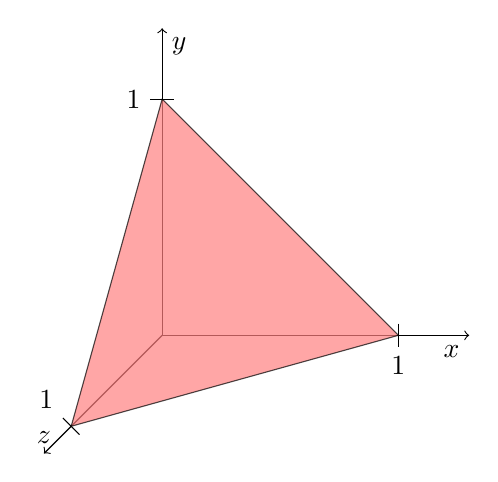
\begin{tikzpicture}[scale=3]
    \begin{scope}
        \draw[->] (0,0,0) -- (1.3,0,0) node[anchor=north east]{$x$};
        \draw[->] (0,0,0) -- (0,1.3,0) node[anchor=north west]{$y$};
        \draw[->] (0,0,0) -- (0,0,1.3) node[anchor=south]{$z$};
        \draw [fill=red!50, opacity=0.7] (0,0,1)--(1,0,0)--(0,1,0)--cycle;
        \draw (1,0.05,0) -- (1,-0.05,0) node[anchor=north]{$1$};
        \draw (0.05,1,0) -- (-0.05,1,0) node[anchor=east] {$1$};
        \draw (0.035,-0.035,1) -- (-0.035,0.035,1) node[anchor=south east]{$1$};
        
    \end{scope}
\end{tikzpicture}

%%% Local Variables: 
%%% mode: latex
%%% TeX-master: "../../main"
%%% End: 

            }
            \caption{Convex Combination.}
        \end{subfigure}
        \label{fig:conservation-gmm}
    \end{figure}
    \begin{align*}
        p(v) = \sum_{h=1}^H\pi_h\cdot\mathcal{N}({v}|\MUH , \SIGMAH )
        % \mathsmaller{p(v)} &= \mathsmaller{\mathcal{N}({v}|\MUH , \SIGMAH )} \\ 
        % &\mathsmaller{= \frac{1}{\sqrt{\det(2\pi\SIGMAH )} }\exp\left(-\frac{1}{2}({v}-\MUH )^\intercal
        %     \left(\SIGMAH\right) ^{-1} ({v}-\MUH )\right)}
    \end{align*}
\end{frame}

\begin{frame}{Merger Resolution}
    \begin{figure}
        \centering
        \scalebox{0.7}{
            \begin{tikzpicture}[minimum size=58pt,scale=0.45, every node/.style={scale=0.45, font=\LARGE}, thick]
                    \begin{scope}
        \node (t1) {\huge $t$};
        \node[hypothesesdetection, below=of t1, circle, draw] (x11) {$X_1^t$};
        \node[hypothesesdetection, below=of x11, circle, draw] (x12) {$X_2^t$};
        \node[hypothesesdetection, below=of x12, circle, draw] (x13) {$X_3^t$};
        \node[hypothesesdetection, below=of x13, circle, draw] (x14) {$X_4^t$};
    \end{scope}
    
    
    \begin{scope}
        \node[right=of t1, xshift=15mm] (t2) {\huge $t+1$};
        \node[hypothesesdetection, below=of t2, circle, draw] (x21) {$X_5^{t+1}$};
        \node[hypothesesdetection, right=of x14, circle, draw, xshift=15mm] (x23) {$X_7^{t+1}$};
        \node[hypothesesdetection, circle, draw] (x22) at ($(x21)!0.5!(x23)$) {$X_6^{t+1}$};
    \end{scope}
    
    \begin{scope}
        \node[right=of t2, xshift=15mm] (t3) {\huge $t+2$};
        \node[hypothesesdetection, below=of t3, circle, draw] (x31) {$X_8^{t+2}$};
        \node[hypothesesdetection, circle, draw, shift=($(x31.center)-(x21.center)$)] (x32) at (x22) {$X_9^{t+2}$};
    \end{scope}
    
    \begin{scope}
        \node[right=of t3, xshift=15mm] (t4) {\huge $t+3$};
        \node[hypothesesdetection, below=of t4, circle, draw] (x41) {$X_{10}^{t+3}$};
        \node[hypothesesdetection, below=of x41, circle, draw] (x42) {$X_{11}^{t+3}$};
        \node[hypothesesdetection, below=of x42, circle, draw] (x43) {$X_{12}^{t+3}$};
        \node[hypothesesdetection, below=of x43, circle, draw] (x44) {$X_{13}^{t+3}$};
    \end{scope}

    \begin{scope}[on background layer]
        \node[rectangle, draw, color=hypothesesbackground!40, fill=hypothesesbackground!30,
        fit=(x11) (x12) (x13) (x14), inner sep=13mm] (b1) {};
        \node[rectangle, draw, color=hypothesesbackground!40, fill=hypothesesbackground!30,
        fit=(x21) (x22) (x23), inner sep=13mm] (b2) {};
        \node[rectangle, draw, color=hypothesesbackground!40, fill=hypothesesbackground!30,
        fit=(b2), shift=($(t3.center) - (t2.center)$), inner sep=-0.1mm] (b3) {};
        \node[rectangle, draw, color=hypothesesbackground!40, fill=hypothesesbackground!30,
        fit=(x41) (x42) (x43) (x44), inner sep=13mm] (b4) {};
    \end{scope}

    \path[hypothesestransition] (x11) edge (x21);
    \path[hypothesestransition] (x12) edge (x22);
    \path[hypothesestransition] (x13) edge (x22);
    \path[hypothesestransition] (x13) edge (x23);
    \path[hypothesestransition] (x14) edge (x23);

    \path[hypothesestransition] (x21) edge (x31);
    \path[hypothesestransition] (x21) edge (x32);
    \path[hypothesestransition] (x22) edge (x32);
    \path[hypothesestransition] (x23) edge (x32);

    \path[hypothesestransition] (x31) edge (x41);
    \path[hypothesestransition] (x32) edge (x42);
    \path[hypothesestransition] (x32) edge (x43);
    \path[hypothesestransition] (x32) edge (x44);

%%% Local Variables: 
%%% mode: latex
%%% TeX-master: "../../../main"
%%% End: 

            \end{tikzpicture}
        }
        \caption{Original hypotheses graph.}
        \label{fig:conservation-hyp-inferred}
    \end{figure}
\end{frame}

\begin{frame}{Merger Resolution}
    \begin{figure}
        \centering
        \scalebox{0.7}{
            \begin{tikzpicture}[minimum size=58pt,scale=0.45, every node/.style={scale=0.45, font=\LARGE}, thick]
                \begin{scope}
    \node (t1) {\huge $t$};
    \node[color=hypothesesoneobject, hypotheses_one_object, below=of t1, circle, draw] (x11) {$X_1^t$};
    \node[color=hypothesesoneobject, hypotheses_one_object, below=of x11, circle, draw] (x12) {$X_2^t$};
    \node[color=hypothesesoneobject, hypotheses_one_object, below=of x12, circle, draw] (x13) {$X_3^t$};
    \node[color=hypothesesoneobject, hypotheses_one_object, below=of x13, circle, draw] (x14) {$X_4^t$};
\end{scope}


\begin{scope}
    \node[right=of t1, xshift=15mm] (t2) {\huge $t+1$};
    \node[color=hypothesesoneobject, hypotheses_one_object, below=of t2, circle, draw] (x21) {$X_5^{t+1}$};
    \node[color=hypothesesoneobject, hypotheses_one_object, right=of x14, circle, draw, xshift=15mm] (x23) {$X_7^{t+1}$};
    \node[color=hypothesestwoobjects, hypotheses_two_objects, circle, draw] (x22) at ($(x21)!0.5!(x23)$) {$X_6^{t+1}$};
\end{scope}

\begin{scope}
    \node[right=of t2, xshift=15mm] (t3) {\huge $t+2$};
    \node[color=hypothesesoneobject, hypotheses_one_object, below=of t3, circle, draw] (x31) {$X_8^{t+2}$};
    \node[color=hypothesesthreeobjects, hypotheses_three_objects, circle, draw, shift=($(x31.center)-(x21.center)$)] (x32) at (x22) {$X_9^{t+2}$};
\end{scope}

\begin{scope}
    \node[right=of t3, xshift=15mm] (t4) {\huge $t+3$};
    \node[color=hypothesesoneobject, hypotheses_one_object, below=of t4, circle, draw] (x41) {$X_{10}^{t+3}$};
    \node[color=hypothesesoneobject, hypotheses_one_object, below=of x41, circle, draw] (x42) {$X_{11}^{t+3}$};
    \node[color=hypothesesoneobject, hypotheses_one_object, below=of x42, circle, draw] (x43) {$X_{12}^{t+3}$};
    \node[color=hypothesesoneobject, hypotheses_one_object, below=of x43, circle, draw] (x44) {$X_{13}^{t+3}$};
\end{scope}

\begin{scope}[on background layer]
    \node[rectangle, draw, color=hypothesesbackground!40, fill=hypothesesbackground!30,
    fit=(x11) (x12) (x13) (x14), inner sep=13mm] (b1) {};
    \node[rectangle, draw, color=hypothesesbackground!40, fill=hypothesesbackground!30,
    fit=(x21) (x22) (x23), inner sep=13mm] (b2) {};
    \node[rectangle, draw, color=hypothesesbackground!40, fill=hypothesesbackground!30,
    fit=(b2), shift=($(t3.center) - (t2.center)$), inner sep=-0.1mm] (b3) {};
    \node[rectangle, draw, color=hypothesesbackground!40, fill=hypothesesbackground!30,
    fit=(x41) (x42) (x43) (x44), inner sep=13mm] (b4) {};
\end{scope}

\path[hypothesestransition] (x11) edge (x21);
\path[hypothesestransition] (x12) edge (x22);
\path[hypothesestransition] (x13) edge (x22);
\path[hypothesestransition] (x14) edge (x23);

\path[hypothesestransition] (x21) edge (x31);
\path[hypothesestransition] (x22) edge (x32);
\path[hypothesestransition] (x23) edge (x32);

\path[hypothesestransition] (x31) edge (x41);
\path[hypothesestransition] (x32) edge (x42);
\path[hypothesestransition] (x32) edge (x43);
\path[hypothesestransition] (x32) edge (x44);

%%% Local Variables: 
%%% mode: latex
%%% TeX-master: "../../../main"
%%% End: 

            \end{tikzpicture}
        }
        \caption{Inferred configuration of the hypotheses graph.}
        \label{fig:conservation-hyp-inferred}
    \end{figure}
\end{frame}

\begin{frame}{Merger Resolution}
    \begin{figure}
        \centering
        \scalebox{0.7}{
            \begin{tikzpicture}[minimum size=58pt,scale=0.45, every node/.style={scale=0.45, font=\LARGE}, thick]
                
\begin{scope}
    \node (t1) {\huge $t$};
    \node[hypothesesdetection, below=of t1, circle, draw] (x11) {$X_2^t$};
    \node[hypothesesdetection, below=of x11, circle, draw] (x12) {$X_3^t$};
\end{scope}


\begin{scope}
    \node[right=of t1, xshift=15mm] (t2) {\huge $t+1$};
    \node[hypotheses_new_detection, below=of t2, circle, draw] (x21) {$X_{14}^{t+1}$};
    \node[hypotheses_new_detection, below=of x21, circle, draw] (x22) {$X_{15}^{t+1}$};
    \node[hypothesesdetection, below=of x22, circle, draw] (x23) {$X_{7}^{t+1}$};
\end{scope}

\begin{scope}
    \node[right=of t2, xshift=15mm] (t3) {\huge $t+2$};
    \node[hypotheses_new_detection, below=of t3, circle, draw] (x31) {$X_{16}^{t+2}$};
    \node[hypotheses_new_detection, below=of x31, circle, draw] (x32) {$X_{17}^{t+2}$};
    \node[hypotheses_new_detection, below=of x32, circle, draw] (x33) {$X_{18}^{t+2}$};
\end{scope}

\begin{scope}
    \node[right=of t3, xshift=15mm] (t4) {\huge $t+3$};
    \node[hypothesesdetection, below=of t4, circle, draw] (x41) {$X_{11}^{t+3}$};
    \node[hypothesesdetection, below=of x41, circle, draw] (x42) {$X_{12}^{t+3}$};
    \node[hypothesesdetection, below=of x42, circle, draw] (x43) {$X_{13}^{t+3}$};
\end{scope}

\begin{scope}[on background layer]
    \node[rectangle, draw, color=hypothesesbackground!40, fill=hypothesesbackground!30,
    fit=(x11) (x12) (x13), inner sep=13mm] (b1) {};
    \node[rectangle, draw, color=hypothesesbackground!40, fill=hypothesesbackground!30,
    fit=(x21) (x22) (x23), inner sep=13mm] (b2) {};
    \node[rectangle, draw, color=hypothesesbackground!40, fill=hypothesesbackground!30,
    fit=(x31) (x32) (x33), inner sep=13mm] (b3) {};
    \node[rectangle, draw, color=hypothesesbackground!40, fill=hypothesesbackground!30,
    fit=(x41) (x42) (x43), inner sep=13mm] (b4) {};
\end{scope}

\path[hypotheses_new_transition] (x11) edge (x21);
\path[hypotheses_new_transition] (x11) edge (x22);


\path[hypotheses_new_transition] (x12) edge (x21);
\path[hypotheses_new_transition] (x12) edge (x22);

\path[hypotheses_new_transition] (x21) edge (x31);
\path[hypotheses_new_transition] (x21) edge (x32);
\path[hypotheses_new_transition] (x21) edge (x33);

\path[hypotheses_new_transition] (x22) edge (x31);
\path[hypotheses_new_transition] (x22) edge (x32);
\path[hypotheses_new_transition] (x22) edge (x33);

\path[hypotheses_new_transition] (x23) edge (x31);
\path[hypotheses_new_transition] (x23) edge (x32);
\path[hypotheses_new_transition] (x23) edge (x33);

\path[hypotheses_new_transition] (x31) edge (x41);
\path[hypotheses_new_transition] (x31) edge (x42);
\path[hypotheses_new_transition] (x31) edge (x43);

\path[hypotheses_new_transition] (x32) edge (x41);
\path[hypotheses_new_transition] (x32) edge (x42);
\path[hypotheses_new_transition] (x32) edge (x43);

\path[hypotheses_new_transition] (x33) edge (x41);
\path[hypotheses_new_transition] (x33) edge (x42);
\path[hypotheses_new_transition] (x33) edge (x43);

%%% Local Variables: 
%%% mode: latex
%%% TeX-master: "../../../main"
%%% End: 

            \end{tikzpicture}
        }
        \caption{Subset of the hypotheses graph that contains all merged objects.}
        \label{fig:conservation-hyp-inferred}
    \end{figure}
\end{frame}

\begin{frame}{Merger Resolution}
    \begin{figure}
        \centering
        \scalebox{0.7}{
            \begin{tikzpicture}[minimum size=58pt,scale=0.45, every node/.style={scale=0.45, font=\LARGE}, thick]
                
\begin{scope}
    \node (t1) {\huge $t$};
    \node[hypotheses_detection_not_involved, below=of t1] (x11) {$X_1^t$};
    \node[hypothesesdetection, below=of x11, circle, draw] (x12) {$X_2^t$};
    \node[hypothesesdetection, below=of x12, circle, draw] (x13) {$X_3^t$};
    \node[hypotheses_detection_not_involved, below=of x13, circle, draw] (x14) {$X_4^t$};
\end{scope}


\begin{scope}
    \node[right=of t1, xshift=15mm] (t2) {\huge $t+1$};
    \node[hypotheses_detection_not_involved, below=of t2] (x21) {$X_5^{t+1}$};
    \node[hypothesesdetection, below=of x21, circle, draw] (x22) {$X_{14}^{t+1}$};
    \node[hypothesesdetection, below=of x22, circle, draw] (x23) {$X_{15}^{t+1}$};
    \node[hypothesesdetection, below=of x23, circle, draw] (x24) {$X_{7}^{t+1}$};
\end{scope}

\begin{scope}
    \node[right=of t2, xshift=15mm] (t3) {\huge $t+2$};
    \node[hypotheses_detection_not_involved, below=of t3] (x31) {$X_8^{t+2}$};
    \node[hypothesesdetection, below=of x31, circle, draw] (x32) {$X_{16}^{t+2}$};
    \node[hypothesesdetection, below=of x32, circle, draw] (x33) {$X_{17}^{t+2}$};
    \node[hypothesesdetection, below=of x33, circle, draw] (x34) {$X_{18}^{t+2}$};
\end{scope}

\begin{scope}
    \node[right=of t3, xshift=15mm] (t4) {\huge $t+3$};
    \node[hypotheses_detection_not_involved, below=of t4] (x41) {$X_{10}^{t+3}$};
    \node[hypothesesdetection, below=of x41, circle, draw] (x42) {$X_{11}^{t+3}$};
    \node[hypothesesdetection, below=of x42, circle, draw] (x43) {$X_{12}^{t+3}$};
    \node[hypothesesdetection, below=of x43, circle, draw] (x44) {$X_{13}^{t+3}$};
\end{scope}

\begin{scope}[on background layer]
    \node[rectangle, draw, color=hypothesesbackground!40, fill=hypothesesbackground!30,
    fit=(x11) (x12) (x13) (x14), inner sep=13mm] (b1) {};
    \node[rectangle, draw, color=hypothesesbackground!40, fill=hypothesesbackground!30,
    fit=(x21) (x22) (x23) (x24), inner sep=13mm] (b2) {};
    \node[rectangle, draw, color=hypothesesbackground!40, fill=hypothesesbackground!30,
    fit=(x31) (x32) (x33) (x34), inner sep=13mm] (b3) {};
    \node[rectangle, draw, color=hypothesesbackground!40, fill=hypothesesbackground!30,
    fit=(x41) (x42) (x43) (x44), inner sep=13mm] (b4) {};
\end{scope}

\path[hypotheses_transition_not_involved] (x11) edge (x21);
\path[hypothesestransition] (x12) edge (x22);
\path[hypothesestransition] (x13) edge (x23);
\path[hypotheses_transition_not_involved] (x14) edge (x24);

\path[hypotheses_transition_not_involved] (x21) edge (x31);
\path[hypothesestransition] (x22) edge (x33);
\path[hypothesestransition] (x23) edge (x32);
\path[hypothesestransition] (x24) edge (x34);

\path[hypotheses_transition_not_involved] (x31) edge (x41);
\path[hypothesestransition] (x32) edge (x42);
\path[hypothesestransition] (x33) edge (x43);
\path[hypothesestransition] (x34) edge (x44);


%%% Local Variables: 
%%% mode: latex
%%% TeX-master: "../../../main"
%%% End: 

            \end{tikzpicture}
        }
        \caption{Inferred configuration of the subset.}
        \label{fig:conservation-hyp-inferred}
    \end{figure}
\end{frame}

% \begin{frame}{Merger Resolution}
%     \begin{figure}
%         \centering
%         \begin{subfigure}{0.3\textwidth}
%             \centering
%             \scalebox{0.65}{
%                 \begin{tikzpicture}[minimum size=58pt,scale=0.45, every node/.style={scale=0.45, font=\LARGE}, thick]
%                         \begin{scope}
        \node (t1) {\huge $t$};
        \node[hypotheses_one_object, below=of t1, circle, draw] (x11) {$X_1^t$};
        \node[hypotheses_one_object, below=of x11, circle, draw] (x12) {$X_2^t$};
    \end{scope}
    \begin{scope}[on background layer]
        \node[hypotheses_division_duplicate, below=of x12, circle, draw, dashed] (x13) {$\bar{X}_2^t$};
    \end{scope}
    
    
    \begin{scope}
        \node[right=of t1, xshift=-6mm] (t2) {\huge $t+1$};
        \node[hypotheses_two_objects, below=of t2, circle, draw] (x21) {$X_3^{t+1}$};
        \node[hypotheses_one_object, below=of x21, circle, draw] (x22) {$X_{4}^{t+1}$};
    \end{scope}
    \begin{scope}[on background layer]
        \node[hypothesesdetection, below=of x22, circle, draw] (x23)  {$X_4^{t+1}$};
    \end{scope}
    
    \begin{scope}
        \node[right=of t2, xshift=-6mm] (t3) {\huge $t+2$};
        \node[hypotheses_one_object, below=of t3, circle, draw] (x31) {$X_5^{t+2}$};
        \node[hypotheses_one_object, below=of x31, circle, draw] (x32) {$X_6^{t+2}$};
        \node[hypotheses_one_object, below=of x32, circle, draw] (x33) {$X_7^{t+2}$};
    \end{scope}
    

    \begin{scope}[on background layer]
        \node[rectangle, draw, color=hypothesesbackground!40, fill=hypothesesbackground!30,
        fit=(x11) (x12) (x13), inner sep=6mm] (b1) {};
        \node[rectangle, draw, color=hypothesesbackground!40, fill=hypothesesbackground!30,
        fit=(x21) (x22) (x23), inner sep=6mm] (b2) {};
        \node[rectangle, draw, color=hypothesesbackground!40, fill=hypothesesbackground!30,
        fit=(x31) (x32) (x33), inner sep=6mm] (b3) {};
    \end{scope}

    \path[hypothesestransition] (x11) edge (x21);
    \path[hypothesestransition] (x12) edge (x21);
    \path[hypothesestransition] (x12) edge (x22);

    \path[hypothesestransition] (x21) edge (x31);
    \path[hypothesestransition] (x21) edge (x32);
    \path[hypothesestransition] (x22) edge (x33);


%%% Local Variables: 
%%% mode: latex
%%% TeX-master: "../../../main"
%%% End: 

%                 \end{tikzpicture}
%             }
%         \end{subfigure}
%         \hfill
%         \begin{subfigure}{0.3\textwidth}
%             \centering
%             \scalebox{0.65}{
%                 \begin{tikzpicture}[minimum size=58pt,scale=0.45, every node/.style={scale=0.45, font=\LARGE}, thick]
%                         \begin{scope}
        \node (t1) {\huge $t$};
        \node[hypothesesdetection, below=of t1, circle, draw] (x11) {$X_1^t$};
        \node[hypotheses_division_duplicate, below=of x11, circle, draw] (x12) {$X_2^t$};
        \node[hypotheses_division_duplicate, below=of x12, circle, draw, dashed] (x13) {$\bar{X}_2^t$};
    \end{scope}
    
    
    \begin{scope}
        \node[right=of t1, xshift=-6mm] (t2) {\huge $t+1$};
        \node[hypotheses_new_detection, below=of t2, circle, draw] (x21) {$X_8^{t+1}$};
        \node[hypotheses_new_detection, below=of x21, circle, draw] (x22) {$X_{9}^{t+1}$};
        \node[hypothesesdetection, below=of x22, circle, draw, dashed] (x23)  {$X_4^{t+1}$};
    \end{scope}
    \begin{scope}[on background layer]
        
    \end{scope}
    
    \begin{scope}
        \node[right=of t2, xshift=-6mm] (t3) {\huge $t+2$};
        \node[hypothesesdetection, below=of t3, circle, draw] (x31) {$X_5^{t+2}$};
        \node[hypothesesdetection, below=of x31, circle, draw] (x32) {$X_6^{t+2}$};
        \node[hypothesesdetection, below=of x32, circle, draw, dashed] (x33) {$X_7^{t+2}$};
    \end{scope}
    

    \begin{scope}[on background layer]
        \node[rectangle, draw, color=hypothesesbackground!40, fill=hypothesesbackground!30,
        fit=(x11) (x12) (x13), inner sep=6mm] (b1) {};
        \node[rectangle, draw, color=hypothesesbackground!40, fill=hypothesesbackground!30,
        fit=(x21) (x22) (x23), inner sep=6mm] (b2) {};
        \node[rectangle, draw, color=hypothesesbackground!40, fill=hypothesesbackground!30,
        fit=(x31) (x32) (x33), inner sep=6mm] (b3) {};
    \end{scope}

    \path[hypotheses_new_transition] (x11) edge (x21);
    \path[hypotheses_new_transition] (x11) edge (x22);
    \path[hypotheses_new_transition] (x12) edge (x21);
    \path[hypotheses_new_transition] (x12) edge (x22);
    \path[hypotheses_new_transition] (x13) edge (x23);

    \path[hypotheses_new_transition] (x21) edge (x31);
    \path[hypotheses_new_transition] (x21) edge (x32);
    \path[hypotheses_new_transition] (x22) edge (x31);
    \path[hypotheses_new_transition] (x22) edge (x32);
    \path[hypotheses_new_transition] (x23) edge (x33);


%%% Local Variables: 
%%% mode: latex
%%% TeX-master: "../../../main"
%%% End: 

%                 \end{tikzpicture}
%             }
%         \end{subfigure}
%         \hfill
%         \begin{subfigure}{0.3\textwidth}
%             \centering
%             \scalebox{0.65}{
%                 \begin{tikzpicture}[minimum size=58pt,scale=0.45, every node/.style={scale=0.45, font=\LARGE}, thick]
%                         \begin{scope}
        \node (t1) {\huge $t$};
        \node[hypothesesdetection, below=of t1, circle, draw] (x11) {$X_1^t$};
        \node[hypothesesdetection, below=of x11, circle, draw] (x12) {$X_2^t$};
    \end{scope}
    \begin{scope}[on background layer]
        \node[hypotheses_division_duplicate, below=of x12, circle, draw, dashed] (x13) {$\bar{X}_2^t$};
    \end{scope}
    
    
    \begin{scope}
        \node[right=of t1, xshift=-6mm] (t2) {\huge $t+1$};
        \node[hypothesesdetection, below=of t2, circle, draw] (x21) {$X_8^{t+1}$};
        \node[hypothesesdetection, below=of x21, circle, draw] (x22) {$X_{9}^{t+1}$};
        \node[hypothesesdetection, below=of x22, circle, draw] (x23)  {$X_4^{t+1}$};
    \end{scope}
    \begin{scope}[on background layer]
        
    \end{scope}
    
    \begin{scope}
        \node[right=of t2, xshift=-6mm] (t3) {\huge $t+2$};
        \node[hypothesesdetection, below=of t3, circle, draw] (x31) {$X_5^{t+2}$};
        \node[hypothesesdetection, below=of x31, circle, draw] (x32) {$X_6^{t+2}$};
        \node[hypothesesdetection, below=of x32, circle, draw] (x33) {$X_7^{t+2}$};
    \end{scope}
    

    \begin{scope}[on background layer]
        \node[rectangle, draw, color=hypothesesbackground!40, fill=hypothesesbackground!30,
        fit=(x11) (x12) (x13), inner sep=6mm] (b1) {};
        \node[rectangle, draw, color=hypothesesbackground!40, fill=hypothesesbackground!30,
        fit=(x21) (x22) (x23), inner sep=6mm] (b2) {};
        \node[rectangle, draw, color=hypothesesbackground!40, fill=hypothesesbackground!30,
        fit=(x31) (x32) (x33), inner sep=6mm] (b3) {};
    \end{scope}

    \path[hypothesestransition] (x11) edge (x21);
    \path[hypothesestransition] (x12) edge (x22);
    \path[hypothesestransition] (x12) edge (x23);

    \path[hypothesestransition] (x21) edge (x31);
    \path[hypothesestransition] (x22) edge (x32);
    \path[hypothesestransition] (x23) edge (x33);


%%% Local Variables: 
%%% mode: latex
%%% TeX-master: "../../../main"
%%% End: 

%                 \end{tikzpicture}
%             }
%         \end{subfigure}
%         \caption{Handling divisions.}
%         \label{fig:conservation-hyp-inferred}
%     \end{figure}
% \end{frame}

\begin{frame}{Merger Resolution - Divisions}
    \begin{figure}
        \centering
        \scalebox{0.8}{
            \begin{tikzpicture}[minimum size=58pt,scale=0.45, every node/.style={scale=0.45, font=\LARGE}, thick]
                    \begin{scope}
        \node (t1) {\huge $t$};
        \node[hypotheses_one_object, below=of t1, circle, draw] (x11) {$X_1^t$};
        \node[hypotheses_one_object, below=of x11, circle, draw] (x12) {$X_2^t$};
    \end{scope}
    \begin{scope}[on background layer]
        \node[hypotheses_division_duplicate, below=of x12, circle, draw, dashed] (x13) {$\bar{X}_2^t$};
    \end{scope}
    
    
    \begin{scope}
        \node[right=of t1, xshift=-6mm] (t2) {\huge $t+1$};
        \node[hypotheses_two_objects, below=of t2, circle, draw] (x21) {$X_3^{t+1}$};
        \node[hypotheses_one_object, below=of x21, circle, draw] (x22) {$X_{4}^{t+1}$};
    \end{scope}
    \begin{scope}[on background layer]
        \node[hypothesesdetection, below=of x22, circle, draw] (x23)  {$X_4^{t+1}$};
    \end{scope}
    
    \begin{scope}
        \node[right=of t2, xshift=-6mm] (t3) {\huge $t+2$};
        \node[hypotheses_one_object, below=of t3, circle, draw] (x31) {$X_5^{t+2}$};
        \node[hypotheses_one_object, below=of x31, circle, draw] (x32) {$X_6^{t+2}$};
        \node[hypotheses_one_object, below=of x32, circle, draw] (x33) {$X_7^{t+2}$};
    \end{scope}
    

    \begin{scope}[on background layer]
        \node[rectangle, draw, color=hypothesesbackground!40, fill=hypothesesbackground!30,
        fit=(x11) (x12) (x13), inner sep=6mm] (b1) {};
        \node[rectangle, draw, color=hypothesesbackground!40, fill=hypothesesbackground!30,
        fit=(x21) (x22) (x23), inner sep=6mm] (b2) {};
        \node[rectangle, draw, color=hypothesesbackground!40, fill=hypothesesbackground!30,
        fit=(x31) (x32) (x33), inner sep=6mm] (b3) {};
    \end{scope}

    \path[hypothesestransition] (x11) edge (x21);
    \path[hypothesestransition] (x12) edge (x21);
    \path[hypothesestransition] (x12) edge (x22);

    \path[hypothesestransition] (x21) edge (x31);
    \path[hypothesestransition] (x21) edge (x32);
    \path[hypothesestransition] (x22) edge (x33);


%%% Local Variables: 
%%% mode: latex
%%% TeX-master: "../../../main"
%%% End: 

            \end{tikzpicture}
        }
    \end{figure}
\end{frame}

\begin{frame}{Merger Resolution - Divisions}
    \begin{figure}
        \centering
        \scalebox{0.8}{
            \begin{tikzpicture}[minimum size=58pt,scale=0.45, every node/.style={scale=0.45, font=\LARGE}, thick]
                    \begin{scope}
        \node (t1) {\huge $t$};
        \node[hypothesesdetection, below=of t1, circle, draw] (x11) {$X_1^t$};
        \node[hypotheses_division_duplicate, below=of x11, circle, draw] (x12) {$X_2^t$};
        \node[hypotheses_division_duplicate, below=of x12, circle, draw, dashed] (x13) {$\bar{X}_2^t$};
    \end{scope}
    
    
    \begin{scope}
        \node[right=of t1, xshift=-6mm] (t2) {\huge $t+1$};
        \node[hypotheses_new_detection, below=of t2, circle, draw] (x21) {$X_8^{t+1}$};
        \node[hypotheses_new_detection, below=of x21, circle, draw] (x22) {$X_{9}^{t+1}$};
        \node[hypothesesdetection, below=of x22, circle, draw, dashed] (x23)  {$X_4^{t+1}$};
    \end{scope}
    \begin{scope}[on background layer]
        
    \end{scope}
    
    \begin{scope}
        \node[right=of t2, xshift=-6mm] (t3) {\huge $t+2$};
        \node[hypothesesdetection, below=of t3, circle, draw] (x31) {$X_5^{t+2}$};
        \node[hypothesesdetection, below=of x31, circle, draw] (x32) {$X_6^{t+2}$};
        \node[hypothesesdetection, below=of x32, circle, draw, dashed] (x33) {$X_7^{t+2}$};
    \end{scope}
    

    \begin{scope}[on background layer]
        \node[rectangle, draw, color=hypothesesbackground!40, fill=hypothesesbackground!30,
        fit=(x11) (x12) (x13), inner sep=6mm] (b1) {};
        \node[rectangle, draw, color=hypothesesbackground!40, fill=hypothesesbackground!30,
        fit=(x21) (x22) (x23), inner sep=6mm] (b2) {};
        \node[rectangle, draw, color=hypothesesbackground!40, fill=hypothesesbackground!30,
        fit=(x31) (x32) (x33), inner sep=6mm] (b3) {};
    \end{scope}

    \path[hypotheses_new_transition] (x11) edge (x21);
    \path[hypotheses_new_transition] (x11) edge (x22);
    \path[hypotheses_new_transition] (x12) edge (x21);
    \path[hypotheses_new_transition] (x12) edge (x22);
    \path[hypotheses_new_transition] (x13) edge (x23);

    \path[hypotheses_new_transition] (x21) edge (x31);
    \path[hypotheses_new_transition] (x21) edge (x32);
    \path[hypotheses_new_transition] (x22) edge (x31);
    \path[hypotheses_new_transition] (x22) edge (x32);
    \path[hypotheses_new_transition] (x23) edge (x33);


%%% Local Variables: 
%%% mode: latex
%%% TeX-master: "../../../main"
%%% End: 

            \end{tikzpicture}
        }
    \end{figure}
\end{frame}

\begin{frame}{Merger Resolution - Divisions}
    \begin{figure}
        \centering
        \scalebox{0.8}{
            \begin{tikzpicture}[minimum size=58pt,scale=0.45, every node/.style={scale=0.45, font=\LARGE}, thick]
                    \begin{scope}
        \node (t1) {\huge $t$};
        \node[hypothesesdetection, below=of t1, circle, draw] (x11) {$X_1^t$};
        \node[hypothesesdetection, below=of x11, circle, draw] (x12) {$X_2^t$};
    \end{scope}
    \begin{scope}[on background layer]
        \node[hypotheses_division_duplicate, below=of x12, circle, draw, dashed] (x13) {$\bar{X}_2^t$};
    \end{scope}
    
    
    \begin{scope}
        \node[right=of t1, xshift=-6mm] (t2) {\huge $t+1$};
        \node[hypothesesdetection, below=of t2, circle, draw] (x21) {$X_8^{t+1}$};
        \node[hypothesesdetection, below=of x21, circle, draw] (x22) {$X_{9}^{t+1}$};
        \node[hypothesesdetection, below=of x22, circle, draw] (x23)  {$X_4^{t+1}$};
    \end{scope}
    \begin{scope}[on background layer]
        
    \end{scope}
    
    \begin{scope}
        \node[right=of t2, xshift=-6mm] (t3) {\huge $t+2$};
        \node[hypothesesdetection, below=of t3, circle, draw] (x31) {$X_5^{t+2}$};
        \node[hypothesesdetection, below=of x31, circle, draw] (x32) {$X_6^{t+2}$};
        \node[hypothesesdetection, below=of x32, circle, draw] (x33) {$X_7^{t+2}$};
    \end{scope}
    

    \begin{scope}[on background layer]
        \node[rectangle, draw, color=hypothesesbackground!40, fill=hypothesesbackground!30,
        fit=(x11) (x12) (x13), inner sep=6mm] (b1) {};
        \node[rectangle, draw, color=hypothesesbackground!40, fill=hypothesesbackground!30,
        fit=(x21) (x22) (x23), inner sep=6mm] (b2) {};
        \node[rectangle, draw, color=hypothesesbackground!40, fill=hypothesesbackground!30,
        fit=(x31) (x32) (x33), inner sep=6mm] (b3) {};
    \end{scope}

    \path[hypothesestransition] (x11) edge (x21);
    \path[hypothesestransition] (x12) edge (x22);
    \path[hypothesestransition] (x12) edge (x23);

    \path[hypothesestransition] (x21) edge (x31);
    \path[hypothesestransition] (x22) edge (x32);
    \path[hypothesestransition] (x23) edge (x33);


%%% Local Variables: 
%%% mode: latex
%%% TeX-master: "../../../main"
%%% End: 

            \end{tikzpicture}
        }
    \end{figure}
\end{frame}

\begin{frame}{Experimental Results}
    \begin{table}
        \centering
        \def\arraystretch{0.5}
\newlength\tablemathtext
\settototalheight\tablemathtext{\parbox{\linewidth}{$t=75$, $\id=446$}}
% \setlength{\tabcolsep}{1pt}
\scalebox{0.95}{
    \begin{tabular}{lccc}
        \toprule
        Time Step \& Id  & Raw Data & Segmentation & GMM fit \\ \midrule
        $t=75$, $\id=446$&
        \raisebox{\tablemathtext-\height}{
            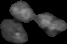
\includegraphics[width=0.18\textwidth]{images/conservation/t=75,id=446,k=3_raw.png}} &
        \raisebox{\tablemathtext-\height}{
            
\includegraphics[width=0.18\textwidth]{images/conservation/t=75,id=446,k=3_label.png}} &
        \raisebox{\tablemathtext-\height}{
            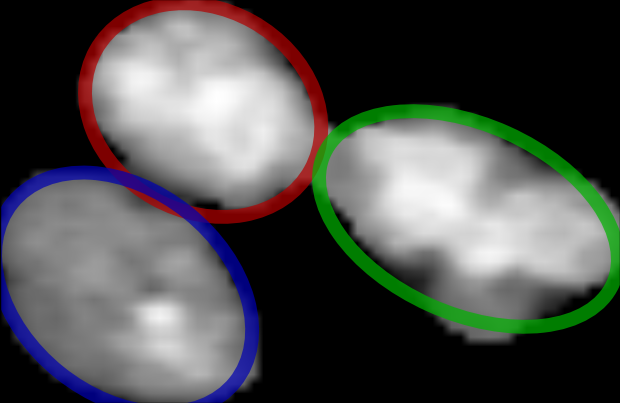
\includegraphics[width=0.18\textwidth]{images/conservation/t=75,id=446,k=3_fit.png}} \\
        &&& \\
        $t=75$, $\id=206$&
        \raisebox{\tablemathtext-\height}{
            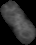
\includegraphics[width=0.18\textwidth]{images/conservation/t=75,id=206,k=2_raw.png}} &
        \raisebox{\tablemathtext-\height}{
            
\includegraphics[width=0.18\textwidth]{images/conservation/t=75,id=206,k=2_label.png}} &
        \raisebox{\tablemathtext-\height}{
            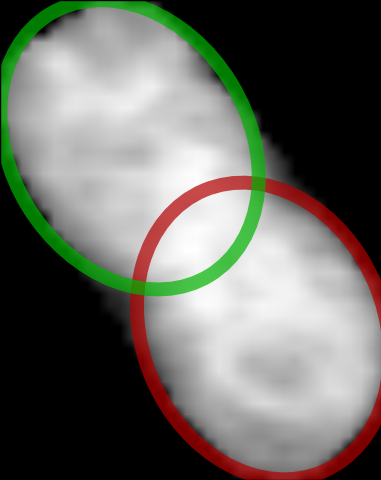
\includegraphics[width=0.18\textwidth]{images/conservation/t=75,id=206,k=2_fit.png}} \\
        &&& \\
        $t=85$, $\id=334$&
        \raisebox{\tablemathtext-\height}{
            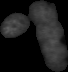
\includegraphics[width=0.18\textwidth]{images/conservation/t=85,id=334,k=4_raw.png}} &
        \raisebox{\tablemathtext-\height}{
            \hspace{-3pt}
\includegraphics[width=0.18\textwidth]{images/conservation/t=85,id=334,k=4_label.png}} &
        \raisebox{\tablemathtext-\height}{
            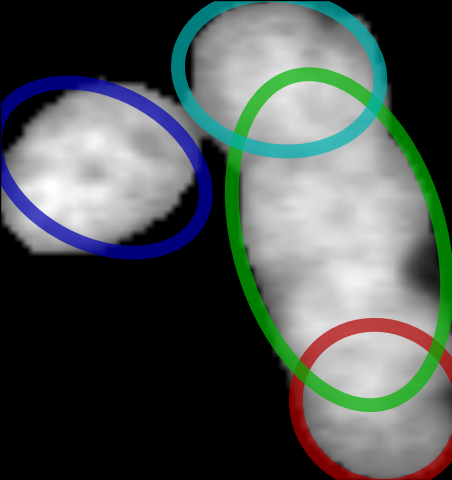
\includegraphics[width=0.18\textwidth]{images/conservation/t=85,id=334,k=4_fit.png}} \\
        \bottomrule
    \end{tabular}
}
\def\arraystretch{1.0}

% WHY THE FUCK THE NEED FOR NEGATIVE HSPACE IN LAST ROW?



%%% Local Variables: 
%%% mode: latex
%%% TeX-master: "../../main"
%%% End: 

        \caption{GMM fits to merged objects.}
        \label{tab:conservation-gmm-fits}
    \end{table}
\end{frame}

% \begin{frame}{Experimental Results}
%     \begin{table} % \small % \hfill{} \centering
%         \scalebox{0.8}{
%             \begin{tabular}{l||ccc|ccc}
%                 \toprule
%                 & \multicolumn{3}{c|}{\textbf{Overall:} 12,289 } & \multicolumn{3}{c}{\textbf{Divisions:} 380 }  \\
%                 & Precision & Recall & $\fmeasure$ &
%                 Precision & Recall & $\fmeasure$    \\
%                 \hline
%                 Kausler \etal & 0.96& 0.96 & 0.96  & 0.92     & 0.91 & 0.92    \\
%                 Classifiers only*				        & \textit{N/A}   & \textit{N/A} & \textit{N/A} & 0.79 & 0.69 & 0.74 \\
%                 Ours ($m=1$)						& 0.94        & 0.95 & 0.94  & 0.92      &
%                 0.88 & 0.90   \\
%                 \bottomrule
%             \end{tabular}
%         }
%         \caption{Results for Drosophila data set 1.}
%         \label{tab:gmm-result-a}
%     \end{table}
% \end{frame}

% \begin{frame}{Experimental Results}
%     \begin{table} % \small % \hfill{} \centering
%         \scalebox{0.8}{
%             \begin{tabular}{l||ccc|ccc}
%                 \toprule
%                 & \multicolumn{3}{c|}{\textbf{Moves}} & \multicolumn{3}{c}{\textbf{Divisions}}  \\
%                 & Precision & Recall & $F_1$& Precision& Recall& $F_{1}$\\
%                 \hline
%                 Kausler \etal 	& 0.92		& 0.92 & 0.92  & 0.05      & 0.12 & 0.06    \\
%                 Classifiers only 	& \textit{N/A}	& \textit{N/A} & \textit{N/A}  & 0.83      & 0.64 & 0.72    \\
%                 Ours ($m=1$)						& 0.97        & 0.95 & 0.96  & 0.62     & 0.63 & 0.63    \\  
%                 Ours ($m=2$)						& 0.97        & 0.97 & 0.97  & 0.53      & 0.79 & 0.64   \\ 
%                 Ours ($m=3$)						& 0.97        & 0.97 & 0.97  & 0.70      & 0.76 & 0.73    \\ 
%                 Ours ($m=4$)						& 0.97        & 0.97 & 0.97  & 0.65      & 0.77 & 0.71    \\ 
%                 \midrule
%                 & \multicolumn{3}{c|}{\textbf{Mergers} } & \multicolumn{3}{c}{\textbf{Resolved Mergers}} \\
%                 & Precision& Recall& $F_{1}$ & Precision& Recall& $F_{1}$ \\
%                 \hline
%                 Kausler \etal & \textit{N/A}& \textit{N/A} & \textit{N/A} & \textit{N/A}& \textit{N/A} & \textit{N/A} \\
%                 Classifiers only & 0.63 & 0.31 & 0.41 & \textit{N/A}& \textit{N/A} & \textit{N/A} \\
%                 Ours ($m=1$) & \textit{N/A}& \textit{N/A} & \textit{N/A} & \textit{N/A}& \textit{N/A} & \textit{N/A}\\
%                 Ours ($m=2$) & 0.71 & 0.54 & 0.61 & 0.72 & 0.61 & 0.66 \\
%                 Ours ($m=3$) & 0.73 & 0.58 & 0.64  & 0.73      & 0.63 & 0.67 \\
%                 Ours ($m=4$) & 0.78      & 0.59 & 0.67 & 0.74      & 0.63 & 0.60 \\
%                 \bottomrule
%             \end{tabular}
%         }
%         \caption{Results for Drosophila data set.}
%         \label{tab:gmm-result-b}
%     \end{table}
% \end{frame}

\begin{frame}{Experimental Results}
    \begin{table} % \small % \hfill{} \centering
        \scalebox{0.8}{
            \begin{tabular}{l||ccc|ccc}
                \toprule
                & \multicolumn{3}{c|}{\textbf{Moves}} & \multicolumn{3}{c}{\textbf{Divisions}} \\
                & Precision& Recall& $\fmeasure$ & Precision& Recall& $\fmeasure$ \\ \hline
                Kausler \etal & 0.99 & 0.97 & 0.98 & 0.65 & 0.68 & 0.66 \\
                Classifiers only & \textit{N/A} & \textit{N/A} & \textit{N/A} & 0.92 & 0.56 & 0.70 \\
                Ours ($m=1$) & 0.99 & 0.97 & 0.98 & 0.68 & 0.71 & 0.70 \\
                Ours ($m=2$) & 1.00 & 0.99 & 0.99 & 0.85 & 0.76 & 0.80 \\
                Ours ($m=3$) & 1.00 & 0.99 & 0.99 & 0.85 & 0.77 & 0.80 \\
                Ours ($m=4$) & 1.00 & 0.99 & 0.99 & 0.85 & 0.76 & 0.80 \\
                \midrule & \multicolumn{3}{c|}{\textbf{Mergers} } & \multicolumn{3}{c}{\textbf{Resolved Mergers}} \\ 
                & Precision& Recall& $F_{1}$ & Precision& Recall& $F_{1}$ \\ \hline
                Kausler \etal & \textit{N/A}& \textit{N/A} & \textit{N/A} & \textit{N/A}&
                \textit{N/A} & \textit{N/A} \\
                Classifiers only & 0.41 & 0.62 & 0.49 & \textit{N/A}& \textit{N/A} & \textit{N/A} \\
                Ours ($m=1$) & \textit{N/A}& \textit{N/A} & \textit{N/A} & \textit{N/A}& \textit{N/A} & \textit{N/A}\\ 
                Ours ($m=2$) & 0.73 & 0.60 & 0.66 & 0.79 & 0.70 & 0.74\\
                Ours ($m=3$) & 0.84 & 0.69 & 0.76 & 0.85 & 0.75 & 0.79\\
                Ours ($m=4$) & 0.84 & 0.69 & 0.76 & 0.85 & 0.75 & 0.80\\
                \bottomrule
            \end{tabular}
        }
        % \caption{Results for Mitocheck data set.}
        \label{tab:gmm-result-c}
    \end{table}
\end{frame}



%%% Local Variables: 
%%% mode: latex
%%% TeX-master: "../main"
%%% End: 
